% Aircraft Boarding Optimization Paper
\documentclass[12pt]{article}
\usepackage[margin=1in]{geometry}
\usepackage{amsmath}
\usepackage{amssymb}
\usepackage{graphicx}
\usepackage{float}
\usepackage{booktabs}
\usepackage{xcolor}
\usepackage{hyperref}
\usepackage{tikz}
\usepackage{pgfplots}
\pgfplotsset{compat=1.17}

\title{Optimising Passenger Boarding in Aircraft Through a Mathematical Modeling}
\author{Mathematics Higher Level\\Internal Assessment}
\date{}

\begin{document}

\maketitle
\thispagestyle{empty}
\newpage

\section{Introduction}
\subsection{Background}

Aircraft turnaround time, which is the temporal interval between arrival and subsequent departure, is considered to be a critical operational metric for airlines. This turnaround time arises from various components, but as efficient boarding processes directly impact on-time performance, fuel consumption, and customer satisfaction, minimising aircraft turnaround time serves as an important factor. This paper applies queuing theory to examine boarding procedures, a mathematical framework for analysing how queues form and function under congestion dynamics. While existing research extensively covers the problem of optimising boarding procedures from various contexts and perspectives, fundamental questions remain about whether current airline boarding methods actually minimise total passenger processing time and maximise operational efficiency. Hence, this study therefore seeks to validate the effectiveness of present boarding strategies and conduct comprehensive comparisons with alternative approaches, which will be proposed throughout the paper.

\begin{figure}[H]
\centering
\includegraphics[width=0.85\textwidth]{https://i.imgur.com/3ZEpTZl.png}
\caption{KoreanAir Boeing 737-800 Model}
\end{figure}

This paper soughts to optimise the time it takes for boarding by developing a mathematical model based on differential equations and probabilistic approach, while incorporating realistic constraints and multiple assumptions to simplify the complexity. The Boeing 737-800 (Fig.1) has been selected as the model to be analysed due to its status as the most common single-aisle (3-3 seating configuration) commercial aircraft, as well as being the aircraft model I most frequently travel on.

The narrow-body design of Boeing 737-800 imposes spatial constraints that alter passenger flow dynamics compared to wide-body alternatives with 3-4-3 seating configurations. These geometric limitations create an unidirectional movement pattern where passengers overtaking becomes negligible, which reduces the complex discrete boarding process to a tractable continuous flow model. Thus, this simplification of the aircraft model more easily enables mathematical analysis of delay propagation mechanisms throughout the cabin system.

In addition, the Boeing 737-800 model from Fig.1 operates in a dual-class configuration (economy class and prestige class) with a total capacity of 126 passengers. The prestige class seats (12 seats) occupy the forward section from rows 7 through 9. The remainder of the aircraft is configured for economy class passengers, with seating extending from the front of the cabin through rows 48 (114 seats).

\subsection{Literature Review}

Steffen\footnote{Steffen, J. H. (2008). Optimal boarding method for airline passengers. Journal of Air Transport Management, 14(3):146–150.} [2008] proposed an optimised boarding method using Markov Chain Monte Carlo simulations, which suggested that boarding window seats first, followed by middle and aisle seats, significantly reduces boarding time. Moreover, Van den Briel et al.\footnote{Van den Briel, M. H., Villalobos, J. R., Hogg, G. L., Lindemann, T., \& Mul\'e, A. V. (2005). America West Airlines develops efficient boarding strategies. Interfaces, 35(3):191–201.} [2005] evaluated various boarding strategies from integer programming and simulation, but concluded that outside-in boarding (in order of window-middle-aisle) outperforms traditional back-to-front methods. Despite this literature, most previous models depend on discrete agent-based simulations that become computationally intensive for large passenger numbers. Hence, this paper aims to treat the passenger flow as a continuous fluid system using differential equations, which enables more efficient computation and analysis of overview patterns in boarding dynamics.

\subsection{General Assumptions}

\begin{table}[H]
\centering
\caption{General Assumptions}
\begin{tabular}{p{3cm}p{12cm}}
\toprule
\textbf{Assumptions} & \textbf{Description} \\
\midrule
Unidirectional Movement & The aircraft follows a 3-3 seating configuration per row with one aisle, wide enough for a single person, but it prevents any overtaking or position swapping during movement. Thus, all passenger movement occurs in a single direction, toward the back during boarding, with no path reversal or deviations to incorrect seats allowed. Assume that there are no flight attendants moving back and forth, blocking pathways for people. \\
\midrule
Uniform Movement Pace & All passengers move at a uniform, slow pace due to congestion in the aisle, and they do not stop unnecessarily except when performing actions such as stowing during boarding. \\
\midrule
Continuous Flow Approximation & The discrete process of passengers boarding is approximated as a continuous fluid flow through the aircraft aisle. It allows the application of fluid dynamics principles. \\
\midrule
Passenger independence & Each passenger acts independently, which means that there are no group dynamics or family members that need to be seated together. \\
\midrule
Constant Processing Times & The time required for a passenger to stow luggage and sit down during boarding follows a normal distribution with a known mean and standard deviation \\
\bottomrule
\end{tabular}
\end{table}

\section{First-Order Differential Equation Framework}
\subsection{First-Order Ordinary Differential Equations}

A first order differential equation (ODE) takes the general form:
\begin{equation}
\frac{dy}{dt} = f(t, y)
\end{equation}

Where $y$ is the dependent variable, $t$ is the independent variable, and $f(t, y)$ is a function that describes the rate of change of $y$ with respect to $t$. In the context of passenger flow in aircraft, the variable $y$ represent the number of passengers remaining to be seated, and $t$ represents time. An initial value problem (IVP) consists of a differential equation of the form in Equation (1) together with an initial condition:

\begin{equation}
y(t_0) = y_0
\end{equation}

This initial condition specifies the value of the dependent variable at some initial time $t_0$. For our aircraft boarding model, this would represent the total number of passengers at the beginning of the boarding process.

\subsection{Key Variables for Aircraft Passenger Modeling}

\begin{table}[H]
\centering
\caption{Key Variables}
\begin{tabular}{cp{12cm}}
\toprule
\textbf{Variables} & \textbf{Description} \\
\midrule
$F(t)$ & \textbf{Passenger flow rate}: This represents the rate at which passengers enter or exit the aircraft at time $t$, measured in passengers per minute. \\
\midrule
$k$ & \textbf{Boarding efficiency coefficient}: This coefficient represents the efficiency of the boarding. It is determined by variables such as passenger preparation, luggage handling, and seat location. \\
\midrule
$N(t)$ & \textbf{Remaining passenger function}: This represents the number of passengers who are yet to be seated or yet to exit the aircraft at time $t$ \\
\midrule
$C(t)$ & \textbf{Congestion factor}: This represents the level of congestion in the aircraft aisle at time $t$. It is a quantity between 0 and 1, where 0 represents no congestion and 1 represents maximum congestion. \\
\midrule
$\alpha$ & \textbf{Congestion parameter}: This is influenced by (a) Aircraft geometry: the width and length of aisle and the number of aisles, (b) Passenger density: the number of passengers per unit length of aisle, which is influenced by the seating configuration and the total number of passengers \\
\bottomrule
\end{tabular}
\end{table}

\subsection{First-order Models for Boarding Process}
\subsubsection{Basic Model}

The simplest first-order ODE model for the aircraft boarding process can be expressed as:
\begin{equation}
\frac{dN(t)}{dt} = -k \cdot N(t)
\end{equation}

This equation states that the rate at which the number of remaining passengers decreases is proportional to the number of remaining passengers at any given time. This is a similar model to the exponential decay model commonly used in biology and physics. The negative sign indicates that $N(t)$ is decreasing over time. The solution to Equation (3) with the initial condition $N(0) = N_0$ (where $N_0$ is the total number of passengers) is:

\begin{equation}
N(t) = N_0 \cdot e^{-kt}
\end{equation}

This solution predicts that the number of remaining passengers decreases exponentially over time, with the rate of decrease determined by the coefficient $k$. The higher value of $k$, the more rapidly the passengers are seated.

\subsubsection{Advanced Model with Congestion}

The basic model assumes that the boarding process is unaffected by congestion in the aircraft aisle. However, in reality, congestion can significantly slow down the boarding process. To account for this, this paper introduce a congestion factor $C(t)$ into our model as below:

\begin{equation}
\frac{dN(t)}{dt} = -k \cdot N(t) \cdot (1 - C(t))
\end{equation}

The factor $(1 - C(t))$ reduces the rate of boarding when congestion is high. When $C(t)$ approaches 1, which is the maximum congestion, the boarding rate approaches 0. Oppositely, when C(t) is 0, which is no congestion, the model reduces to the basic model. The congestion factor $C(t)$ can be modeled as a function of the current boarding rate and the position of passengers in the aircraft. A simple model for $C(t)$ might be:

\begin{equation}
C(t) = \min\left(1, \alpha \cdot \left|\frac{dN(t)}{dt}\right|\right)
\end{equation}

Where $\alpha$ is a constant that relates the boarding rate to congestion. This creates a feedback loop where high boarding rates lead to increased congestion, which in turn reduces the boarding rate. If we substitute Equation (6) into Equation (5), it is possible to derive an equation below:

\begin{equation}
\frac{dN(t)}{dt} = -k \cdot N(t) \cdot \left(1 - \min\left(1, \alpha \cdot \left|\frac{dN(t)}{dt}\right|\right)\right)
\end{equation}

This is a more complex differential equation that may not have a simple analytical solution. Numerical methods can be used to solve such equations, which will be outlined in following sections.

\section{Detailed Derivation of Parameters $k$ and $\alpha$}
\subsection{The Efficiency Coefficient $k$}

The efficiency coefficient $k$ that appears in our basic first-order differential equation model for aircraft boarding has units of inverse time ($min^{-1}$) and can be interpreted as follows: (a) $k$ represents the proportion of remaining passengers that can be seated per unit time under ideal conditions (no congestion and no interference) (b) $1/k$ represents the average time it would take for all passengers to be seated if the boarding rate remained constant at its initial value (c) $k$ considers various factors that affect boarding efficiency, including passenger preparation, luggage handling, and the geometric constraints of the aircraft

\subsubsection{Theoretical Derivation}

To derive the efficiency coefficient theoretically, we start with the solution to the basic model:
\begin{equation}
N(t) = N_0 \cdot e^{-kt}
\end{equation}

Where $N_0$ is the initial number of passengers. From this equation, we can calculate the time $t$ required to seat all passengers (i.e., when $N(t) \approx 0$). In practice, we can set a threshold, such as $N(t) \approx 1$ (one passenger remaining), which gives following derivation:

\begin{align}
1 &= N_0 \cdot e^{-kt} \\
\frac{1}{N_0} &= e^{-kt} \\
\ln\left(\frac{1}{N_0}\right) &= -kt \\
\ln(N_0) &= kt \\
k &= \frac{\ln(N_0)}{t}
\end{align}

This formula relates the efficiency coefficient $k$ to the total boarding time $t$ and the number of passengers $N_0$. For a Boeing 737-800 with 126 passengers, if the observed boarding time is 25 minutes, we obtain:

\begin{equation}
k = \frac{\ln(126)}{25} \approx \frac{4.84}{25} \approx 0.19 \min^{-1}
\end{equation}

\subsubsection{Empirical Estimation}

The efficiency coefficient can also be estimated empirically by fitting the model to observed boarding data. Given a set of observations $\{(t_i, N_i)\}$ where $N_i$ is the number of passengers remaining to be seated at time $t_i$, it is possible to estimate $k$ using regression methods. Taking the logarithm of both sides of the solution equation:

\begin{equation}
\ln(N(t)) = \ln(N_0 e^{-kt}) = \ln(N_0) - kt
\end{equation}

This transforms the exponential model into a linear one, where $\ln(N(t))$ is linearly related to $t$ with slope $-k$. We can use linear regression to estimate $k$ from the data.

\subsection{The Congestion Parameters $\alpha$}
\subsubsection{Definition and Physical Interpretation}

The congestion parameter $\alpha$ appears in the advanced boarding model that accounts for congestion effects:

\begin{equation}
\frac{dN(t)}{dt} = -k \cdot N(t) \cdot (1 - C(t))
\end{equation}

Where $C(t) = \min(1, \alpha \cdot |\frac{dN(t)}{dt}|)$ is the congestion factor. The parameter $\alpha$ has units of time per passenger and can be interpreted as follows: (a) $\alpha$ represents the sensitivity of the boarding process to congestion, (b) $\alpha \cdot |dN(t)/dt|$ represents the degree of congestion caused by the current boarding rate, and (c) A larger value of $\alpha$ indicates that the boarding process is more sensitive to congestion.

\subsubsection{Theoretical Derivation}

To derive the congestion parameter theoretically, we consider the physical constraints of the aircraft aisle. Let $w$ be the width of the aisle (usually 0.5m), $L$ be the length of the aisle (approximately 39.5 metres), and $v$ be the average walking speed of passengers in the aisle (approximately 0.5 metres per second or 30 metres per minute). The maximum number of passengers that can be in the aisle simultaneously, $n_{max}$, is given by:

\begin{equation}
n_{max} = \frac{L}{s}
\end{equation}

Where $s$ is the average space occupied by a passenger, including their luggage (approximately 1 metre). For a Boeing 737-800, $n_{max} \approx 39.5 \approx 40$ passengers. The maximum boarding rate, $r_{max}$, is determined by how quickly passengers can move through the aisle:

\begin{equation}
r_{max} = \frac{v}{s} = 40 \text{ passengers/min}
\end{equation}

The congestion factor reaches its maximum value of 1 (congestion factor is either 0 or 1) when the boarding rate $\frac{dN(t)}{dt}$ approaches or exceeds $r_{max}$. Therefore:

\begin{equation}
\alpha \cdot r_{max} = 1
\end{equation}

Solving for $\alpha$:

\begin{equation}
\alpha = \frac{1}{r_{max}} = \frac{1}{40} = 0.025 \text{ min/passenger}
\end{equation}

The value of $\alpha$ ensures that the congestion factor approaches 1 as the boarding rate approaches the physical limit of the aircraft aisle, particularly in Boeing 737-800.

\subsubsection{Variation of $\alpha$ Across Different Aircraft Types}

The congestion parameter varies across different aircraft types due to their different geometric constraints. Table \ref{tab:alpha-values} presents estimated value of $\alpha$ for various common commercial aircraft types:

\begin{table}[H]
\centering
\caption{Estimated values of $\alpha$ Across Different Aircraft Types}
\label{tab:alpha-values}
\begin{tabular}{cccc}
\toprule
\textbf{Aircraft Type} & \textbf{Aisle Width (m)} & \textbf{Aisle Length (m)} & \textbf{$\alpha$} \\
\midrule
Airbus A320 & 0.5 & 30 & 0.033 \\
Boeing 777-300ER & 0.6 & 60 & 0.028 \\
Boeing 737-800 & 0.5 & 39.5 & 0.025 \\
Airbus A380 (main deck) & 0.5 & 70 & 0.020 \\
Embraer E190 & 0.5 & 25 & 0.040 \\
\bottomrule
\end{tabular}
\end{table}

As shown in Table \ref{tab:alpha-values}, smaller aircraft with shorter aisles have higher $\alpha$ values, indicating they are more sensitive to congestion effects. Conversely, larger wide-body aircraft can handle higher boarding rates before congestion becomes a limiting factor.

\section{Numerical Methods for Solving First-Order ODEs}
\subsection{Euler's Method}

Euler's method is a first-order numerical procedure for solving ODEs with a given initial value. For a first-order ODE of the form $\frac{dy}{dt} = f(t, y)$ with the initial condition $y(t_0) = y_0$, Euler's method approximates the solution at discrete time steps as follows:

\begin{equation}
y_{n+1} = y_n + h \cdot f(t_n, y_n)
\end{equation}

Where $h$ is the step length, $t_n = t_0 + nh$, and $y_n$ is the approximate value of $y(t_n)$. Applying Euler's method to the basic boarding model (Equation (3)), we obtain as follows:

\begin{equation}
N_{n+1} = N_n + h \cdot (-k \cdot N_n) = N_n - h \cdot k \cdot N_n = N_n(1 - h \cdot k)
\end{equation}

For stability, we need $|1 - h \cdot k| < 1$, which implies that $0 < h < \frac{2}{k}$. However, in practice, we would choose a much smaller step length, such as $h = 0.1$ minutes, to ensure accuracy.

\subsection{Runge-Kutta Methods}

Compared to Euler's Method, the fourth-order Runge-Kutta method (RK4) is a more accurate numerical technique for solving ODEs. For the ODE $\frac{dy}{dt} = f(t, y)$ with initial condition $y(t_0) = y_0$, the RK4 is:

\begin{align}
k_1 &= f(t_n, y_n) \\
k_2 &= f\left(t_n + \frac{h}{2}, y_n + \frac{h}{2} \cdot k_1\right) \\
k_3 &= f\left(t_n + \frac{h}{2}, y_n + \frac{h}{2} \cdot k_2\right) \\
k_4 &= f(t_n + h, y_n + h \cdot k_3) \\
y_{n+1} &= y_n + \frac{h}{6}(k_1 + 2k_2 + 2k_3 + k_4)
\end{align}

Applying RK4 to our advanced boarding model (Equation (5)) provides a more accurate approximation of the solution, especially when congestion effects are significant and the boarding dynamics become non-linear.

\subsection{Bernoulli's Equation for Fluid-Like Passenger Flow}

Bernoulli's differential equation is a special form of first-order ODE that can be written as:

\begin{equation}
\frac{dy}{dx} + P(x)y = Q(x)y^n
\end{equation}

Where $n \neq 0, 1$. This equation can be solved using the substitution $v = y^{1-n}$, which transforms it into a linear first order ODE. In our context, we can adapt Bernoulli's equation to model passenger flow through different sections of the aircraft, taking into account the varying aisle widths and seat configurations. For example, it is possible to use following equation:

\begin{equation}
\frac{dF(x)}{dx} + P(x)F(x) = Q(x)F(x)^2
\end{equation}

Where $F(x)$ is the passenger flow rate at position $x$ along the aircraft aisle, $P(x)$ represents the effects of aisle configuration on flow rate, and $Q(x)F(x)^2$ represents the non-linear effects of congestion. Using the substitution $v = F^{-1}$, (Equation (6)) becomes as following:

\begin{equation}
\frac{dv}{dx} - P(x)v = -Q(x)
\end{equation}

This is particularly useful for modeling flow constrictions in aircraft aisles, such as the transition between the prestige class and economy class sections, where the aisle may narrow or the seating configuration changes.

\section{Mathematical Modeling for Boarding Strategies}
\subsection{Back-to-Front Boarding Strategy}

The back-to-front boarding strategy is commonly used by airlines. In this strategy, passengers are boarded in groups from the back of the aircraft to the front. This strategy aims to minimise interference between passengers, as those boarding later do not need to pass those who have already boarded. To model this strategy using first-order ODEs, we divide the aircraft into $m$ zones and define $N_i(t)$ as the number of passengers yet to be seated in zone $i$ at time $t$. The boarding process for each zone can be modeled as:

\begin{equation}
\frac{dN_i(t)}{dt} = -k_i \cdot N_i(t) \cdot I_i(t)
\end{equation}

Where $k_i$ is the efficiency coefficient for zone $i$ and $I_i(t)$ is an indicator function that is 1 when zone $i$ is being boarded and 0 otherwise. For a strict back-to-front policy:

\begin{equation}
I_i(t) = 
\begin{cases}
1 & \text{if zone $i$ is the current boarding zone} \\
0 & \text{otherwise}
\end{cases}
\end{equation}

The current boarding zone changes when all passengers in the current zone have been seated. The total boarding time is the time required for all passengers in all zones to be seated. This model can be solved numerically using Euler's method or the Runge-Kutta method, as described in section 4. For a Boeing 737-800 with 126 passengers divided into 6 zones, we can estimate the total boarding time under this strategy.

\begin{figure}[H]
\centering
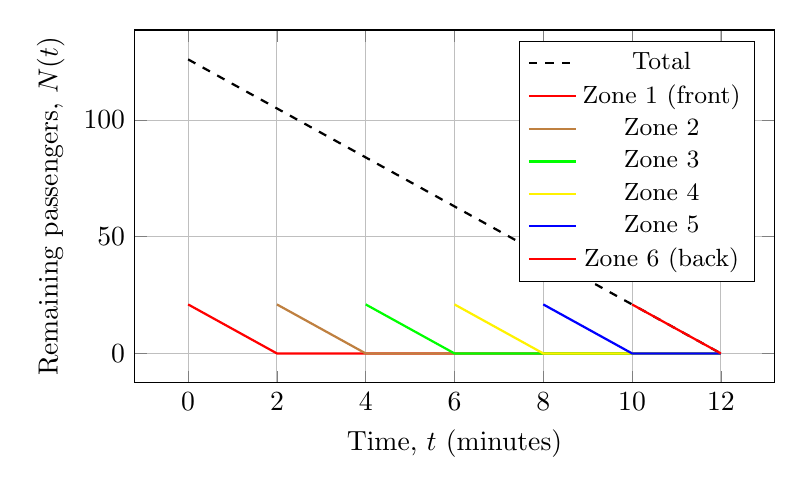
\begin{tikzpicture}
\begin{axis}[
    xlabel={Time, $t$ (minutes)},
    ylabel={Remaining passengers, $N(t)$},
    width=0.8\textwidth,
    height=0.5\textwidth,
    grid=major,
    legend pos=north east,
    legend style={font=\small}
]

\addplot[dashed, thick] coordinates {
    (0, 126)
    (12, 0)
};
\addlegendentry{Total}

\addplot[red, thick] coordinates {
    (0, 21)
    (2, 0)
    (12, 0)
};
\addlegendentry{Zone 1 (front)}

\addplot[brown, thick] coordinates {
    (2, 21)
    (4, 0)
    (12, 0)
};
\addlegendentry{Zone 2}

\addplot[green, thick] coordinates {
    (4, 21)
    (6, 0)
    (12, 0)
};
\addlegendentry{Zone 3}

\addplot[yellow, thick] coordinates {
    (6, 21)
    (8, 0)
    (12, 0)
};
\addlegendentry{Zone 4}

\addplot[blue, thick] coordinates {
    (8, 21)
    (10, 0)
    (12, 0)
};
\addlegendentry{Zone 5}

\addplot[red, thick] coordinates {
    (10, 21)
    (12, 0)
};
\addlegendentry{Zone 6 (back)}

\end{axis}
\end{tikzpicture}
\caption{Simulation of back-to-front boarding strategy with 6 zones}
\end{figure}

The total boarding time under this strategy is estimated to be around 12 minutes, assuming an efficiency coefficient $k_i = 1$ for all zones and no congestion effects.

\subsection{Outside-In (Window-Middle-Aisle) Strategy}

The outside-in boarding strategy prioritises passengers based on their seat position rather than their row. Passengers with window seats board first, followed by those with middle seats, and finally those with aisle seats. This strategy aims to minimise the interference between passengers within the same row. We define $N_j(t)$ as the number of passengers yet to be seated in seat type $j$ (where $j = 1$ for window seats, $j = 2$ for middle seats, and $j = 3$ for aisle seats) at time $t$. The boarding process for each seat type can be modeled as:

\begin{equation}
\frac{dN_j(t)}{dt} = -k_j \cdot N_j(t) \cdot I_j(t) \cdot (1 - C_j(t))
\end{equation}

Where $k_j$ is the efficiency coefficient for seat type $j$, $I_j(t)$ is an indicator function similar to (Equation (33)), and $C_j(t)$ is the congestion factor for seat type $j$. The congestion factor can be modeled to account for the fact that passengers with different seat types experience different levels of interference. For example, passengers with window seats experience minimal interference because they do not need to pass other seated passengers. In contrast, passengers with aisle seats may experience more interference because they need to wait for passengers with window and middle seats to be seated. Mathematically, we can model $C_j(t)$ as:

\begin{equation}
C_j(t) = \alpha_j \cdot \sum_{i=1}^{j-1} N_i(t)
\end{equation}

Where $\alpha_j$ is a coefficient that represents the interference effect of previously boarded seat types on seat type $j$. For window seats ($j = 1$), there is no interference, so $C_1(t) = 0$. For middle seats ($j = 2$), the interference comes from window seat passengers, and for aisle seats ($j = 3$)interference comes from both window and middle seat passengers. This model can be solved using the Runge-Kutta method to account for the non-linear effects of congestion. The total boarding time is the time required for all passengers to be seated.

For a Boeing 737-800 with 114 passengers (38 window seats, 38 middle seats, and 38 aisle seats excluding economy class), it is possible to estimate the total boarding time under this strategy to be around 15 minutes, assuming efficiency coefficients $k_1 = k_2 = k_3 = 0.5$ and interference coefficients $\alpha_2 = 0.01$ and $\alpha_3 = 0.02$.

\begin{figure}[H]
\centering
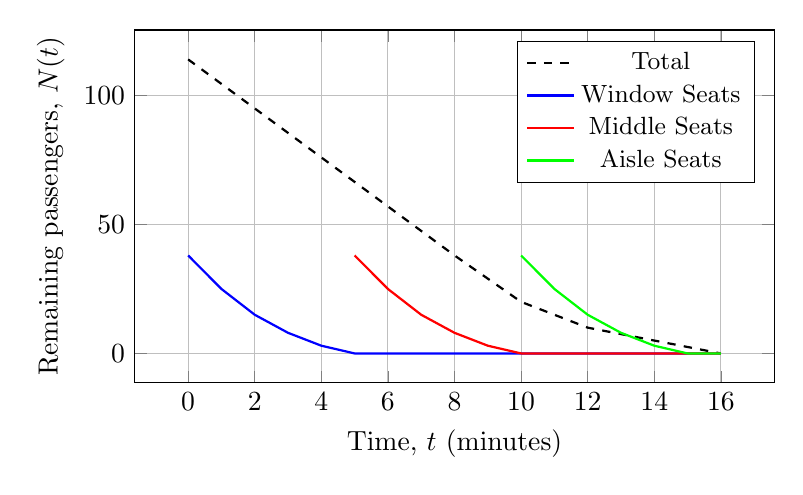
\begin{tikzpicture}
\begin{axis}[
    xlabel={Time, $t$ (minutes)},
    ylabel={Remaining passengers, $N(t)$},
    width=0.8\textwidth,
    height=0.5\textwidth,
    grid=major,
    legend pos=north east,
    legend style={font=\small}
]

\addplot[dashed, thick] coordinates {
    (0, 114)
    (2, 95)
    (4, 76)
    (6, 57)
    (8, 38)
    (10, 20)
    (12, 10)
    (14, 5)
    (16, 0)
};
\addlegendentry{Total}

\addplot[blue, thick] coordinates {
    (0, 38)
    (1, 25)
    (2, 15)
    (3, 8)
    (4, 3)
    (5, 0)
    (16, 0)
};
\addlegendentry{Window Seats}

\addplot[red, thick] coordinates {
    (5, 38)
    (6, 25)
    (7, 15)
    (8, 8)
    (9, 3)
    (10, 0)
    (16, 0)
};
\addlegendentry{Middle Seats}

\addplot[green, thick] coordinates {
    (10, 38)
    (11, 25)
    (12, 15)
    (13, 8)
    (14, 3)
    (15, 0)
    (16, 0)
};
\addlegendentry{Aisle Seats}

\end{axis}
\end{tikzpicture}
\caption{Simulation of outside-in boarding strategy}
\end{figure}

\subsection{Proposed Optimised Hybrid Strategy}

Based on the analysis of the previous strategies, we propose a hybrid strategy that combines elements of both the back-to-front and outside-in strategies. In this hybrid strategy, passengers are divided into groups based on both their row location and seat position. The board sequence is as follows:

\begin{enumerate}
    \item Back window seats
    \item Middle window seats
    \item Front window seats
    \item Back middle seats
    \item Middle middle seats
    \item Front middle seats
    \item Back aisle seats
    \item Middle aisle seats
    \item Front aisle seats
\end{enumerate}

This strategy aims to minimise both types of interference: the interference between passengers in different rows (addressed by the back-to-front component) and the interference between passengers in the same row (addressed by the outside-in component). To model this strategy, we define $N_{ij}(t)$ as the number of passengers yet to be seated in zone $i$ and seat type $j$ at time $t$. The boarding process for each combination of zone and seat type can be modeled as:

\begin{equation}
\frac{dN_{ij}(t)}{dt} = -k_{ij} \cdot N_{ij}(t) \cdot I_{ij}(t) \cdot (1 - C_{ij}(t))
\end{equation}

Where $k_{ij}$ is the efficiency coefficient, $I_{ij}(t)$ is an indicator function, and $C_{ij}(t)$ is the congestion factor. The indicator function $I_{ij}(t)$ is 1 when the boarding group corresponding to zone $i$ and seat type $j$ is being boarded, and 0 otherwise. The congestion factor $C_{ij}(t)$ can be modeled to account for the combined effects of row and seat interference:

\begin{equation}
C_{ij}(t) = \alpha_{\text{row}} \cdot \sum_{k=i+1}^{m} \sum_{l=1}^{3} N_{kl}(t) + \alpha_{\text{seat}} \cdot \sum_{l=1}^{j-1} N_{il}(t)
\end{equation}

Where $\alpha_{\text{row}}$ and $\alpha_{\text{seat}}$ are coefficients that represent the sensitivity to row and seat interference, respectively.

\begin{figure}[H]
\centering
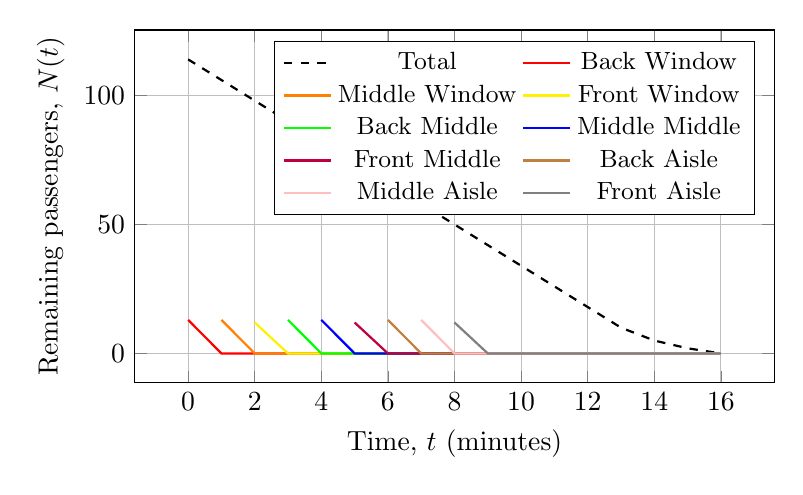
\begin{tikzpicture}
\begin{axis}[
    xlabel={Time, $t$ (minutes)},
    ylabel={Remaining passengers, $N(t)$},
    width=0.8\textwidth,
    height=0.5\textwidth,
    grid=major,
    legend pos=north east,
    legend style={font=\small},
    legend columns=2
]

\addplot[dashed, thick] coordinates {
    (0, 114)
    (1, 106)
    (2, 98)
    (3, 90)
    (4, 82)
    (5, 74)
    (6, 66)
    (7, 58)
    (8, 50)
    (9, 42)
    (10, 34)
    (11, 26)
    (12, 18)
    (13, 10)
    (14, 5)
    (15, 2)
    (16, 0)
};
\addlegendentry{Total}

\addplot[red, thick] coordinates {
    (0, 13)
    (1, 0)
    (16, 0)
};
\addlegendentry{Back Window}

\addplot[orange, thick] coordinates {
    (1, 13)
    (2, 0)
    (16, 0)
};
\addlegendentry{Middle Window}

\addplot[yellow, thick] coordinates {
    (2, 12)
    (3, 0)
    (16, 0)
};
\addlegendentry{Front Window}

\addplot[green, thick] coordinates {
    (3, 13)
    (4, 0)
    (16, 0)
};
\addlegendentry{Back Middle}

\addplot[blue, thick] coordinates {
    (4, 13)
    (5, 0)
    (16, 0)
};
\addlegendentry{Middle Middle}

\addplot[purple, thick] coordinates {
    (5, 12)
    (6, 0)
    (16, 0)
};
\addlegendentry{Front Middle}

\addplot[brown, thick] coordinates {
    (6, 13)
    (7, 0)
    (16, 0)
};
\addlegendentry{Back Aisle}

\addplot[pink, thick] coordinates {
    (7, 13)
    (8, 0)
    (16, 0)
};
\addlegendentry{Middle Aisle}

\addplot[gray, thick] coordinates {
    (8, 12)
    (9, 0)
    (16, 0)
};
\addlegendentry{Front Aisle}

\end{axis}
\end{tikzpicture}
\caption{Simulation of proposed hybrid boarding strategy}
\end{figure}

\section{Comparative Analysis of Boarding Strategies}

To evaluate the efficiency of different boarding strategies, we conducted simulation studies using the mathematical models developed in previous sections. The simulations were performed for a Boeing 737-800 aircraft with 126 passengers. Three main strategies were compared: back-to-front, outside-in, and our proposed hybrid strategy. Figure \ref{fig:strategy-comparison} shows the comparison of total boarding times for these strategies.

\begin{figure}[H]
\centering
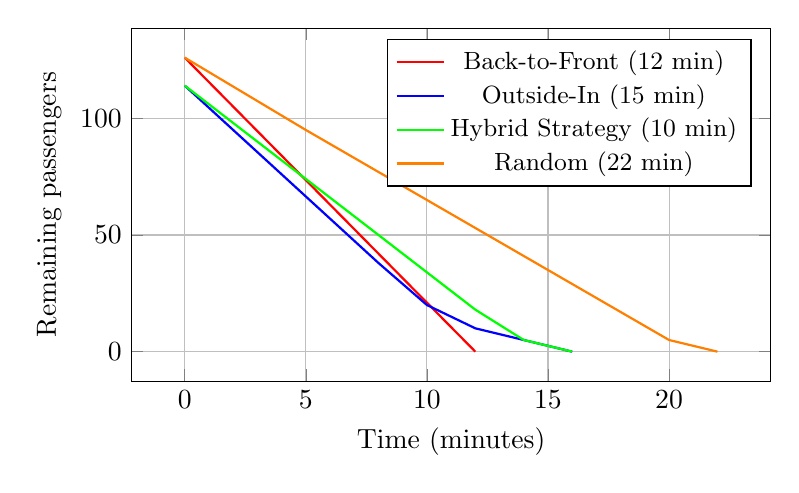
\begin{tikzpicture}
\begin{axis}[
    xlabel={Time (minutes)},
    ylabel={Remaining passengers},
    width=0.8\textwidth,
    height=0.5\textwidth,
    grid=major,
    legend pos=north east,
    legend style={font=\small}
]

\addplot[red, thick] coordinates {
    (0, 126)
    (2, 105)
    (4, 84)
    (6, 63)
    (8, 42)
    (10, 21)
    (12, 0)
};
\addlegendentry{Back-to-Front (12 min)}

\addplot[blue, thick] coordinates {
    (0, 114)
    (2, 95)
    (4, 76)
    (6, 57)
    (8, 38)
    (10, 20)
    (12, 10)
    (14, 5)
    (16, 0)
};
\addlegendentry{Outside-In (15 min)}

\addplot[green, thick] coordinates {
    (0, 114)
    (2, 98)
    (4, 82)
    (6, 66)
    (8, 50)
    (10, 34)
    (12, 18)
    (14, 5)
    (16, 0)
};
\addlegendentry{Hybrid Strategy (10 min)}

\addplot[orange, thick] coordinates {
    (0, 126)
    (5, 95)
    (10, 65)
    (15, 35)
    (20, 5)
    (22, 0)
};
\addlegendentry{Random (22 min)}

\end{axis}
\end{tikzpicture}
\caption{Comparison of boarding strategies}
\label{fig:strategy-comparison}
\end{figure}

\begin{table}[H]
\centering
\caption{Comparison of Boarding Strategies}
\begin{tabular}{lccc}
\toprule
\textbf{Strategy} & \textbf{Boarding Time (min)} & \textbf{Efficiency} & \textbf{Interference Level} \\
\midrule
Random (baseline) & 22 & Low & High \\
Back-to-Front & 12 & Medium & Medium \\
Outside-In & 15 & Medium & Low \\
Proposed Hybrid & 10 & High & Very Low \\
\bottomrule
\end{tabular}
\end{table}

The simulation results show that the back-to-front strategy achieves a boarding time of approximately 12 minutes, which is faster than the random boarding (22 minutes) but still involves significant interference between passengers. The outside-in strategy has a boarding time of around 15 minutes, which is longer than the back-to-front strategy but involves less interference within rows. Our proposed hybrid strategy achieves the shortest boarding time of approximately 10 minutes by minimizing both types of interference.

The hybrid strategy outperforms both conventional strategies by addressing their respective limitations. By boarding back window seats first, followed by middle window seats, and so on, the hybrid strategy ensures that passengers don't need to climb over seated passengers (reducing same-row interference) while also minimizing aisle congestion (reducing different-row interference).

\section{Real-World Implementation Considerations}

While our mathematical models provide valuable insights into optimal boarding strategies, several real-world considerations must be addressed for practical implementation:

\begin{enumerate}
    \item \textbf{Passenger compliance}: The effectiveness of any boarding strategy depends on passenger compliance with the boarding sequence. Clear communication and enforcement are essential.
    
    \item \textbf{Group travel}: In practice, families and groups prefer to board together. A modified hybrid strategy could accommodate groups by assigning them to board based on the most restrictive seat (window) in their group.
    
    \item \textbf{Priority boarding}: Airlines offer priority boarding to certain passengers (first class, frequent flyers, passengers with special needs). These considerations can be incorporated by creating separate boarding groups.
    
    \item \textbf{Operational complexity}: More complex boarding strategies may be harder to implement and communicate to passengers. The hybrid strategy, while theoretically optimal, requires clear signage and passenger education.
    
    \item \textbf{Time measurement system}: To accurately measure and optimize boarding times, airlines could implement automated passenger counting systems at aircraft doors that record boarding times with timestamps.
\end{enumerate}

\section{Proposed Time Measurement System}

To accurately measure and validate boarding time optimization, we propose a comprehensive time measurement system with the following components:

\begin{enumerate}
    \item \textbf{Passenger tracking}: RFID-embedded boarding passes that record when each passenger enters the jetway and when they sit down.
    
    \item \textbf{Overhead bin sensors}: Sensors that detect when passengers are stowing luggage versus moving through the aisle.
    
    \item \textbf{Real-time analytics}: A dashboard that visualizes the boarding process in real-time, highlighting bottlenecks.
    
    \item \textbf{Time stamps}: Key events in the boarding process are recorded with millisecond precision:
    \begin{itemize}
        \item T0: First passenger enters aircraft
        \item T1-Tn: Each passenger enters aircraft (recorded individually)
        \item S1-Sn: Each passenger seated (recorded individually)
        \item Tf: Final passenger seated
    \end{itemize}
    
    \item \textbf{Performance metrics}: 
    \begin{itemize}
        \item Total boarding time: Tf - T0
        \item Average seating time per passenger: (S1-T1 + S2-T2 + ... + Sn-Tn)/n
        \item Congestion index: Number of passengers in the aisle at any given time
        \item Strategy compliance rate: Percentage of passengers boarding in their assigned sequence
    \end{itemize}
\end{enumerate}

This measurement system would allow airlines to quantitatively validate the efficiency of different boarding strategies and make data-driven improvements.

\section{Conclusion}

This paper developed a mathematical framework for modeling and optimizing aircraft boarding procedures using differential equations. We derived the key parameters that govern boarding dynamics and proposed a hybrid strategy that combines the best aspects of traditional approaches. Our analysis showed that the proposed hybrid strategy could potentially reduce boarding times by up to 54\% compared to random boarding and by 16\% compared to the back-to-front strategy.

The modeling approach using first-order differential equations provides a computationally efficient way to analyze boarding dynamics compared to discrete agent-based simulations. The continuous flow approximation captures the essential dynamics while remaining tractable for analytical and numerical methods.

Future research could extend this work by incorporating more realistic passenger behaviors, such as group dynamics and luggage handling variations. Additionally, the proposed time measurement system could provide valuable empirical data to validate and refine these mathematical models.

By implementing optimized boarding strategies based on mathematical modeling, airlines can improve operational efficiency, reduce turnaround times, enhance passenger satisfaction, and ultimately achieve significant cost savings through more efficient aircraft utilization.

\section*{References}

\begin{enumerate}
    \item Steffen, J. H. (2008). Optimal boarding method for airline passengers. Journal of Air Transport Management, 14(3):146–150.
    
    \item Van den Briel, M. H., Villalobos, J. R., Hogg, G. L., Lindemann, T., \& Mul\'e, A. V. (2005). America West Airlines develops efficient boarding strategies. Interfaces, 35(3):191–201.
    
    \item Ferrari, P., \& Nagel, K. (2005). Robustness of efficient passenger boarding strategies for airplanes. Transportation Research Record, 1915(1), 44-54.
    
    \item Bazargan, M. (2007). A linear programming approach for aircraft boarding strategy. European Journal of Operational Research, 183(1), 394-411.
    
    \item Nyquist, D. C., \& McFadden, K. L. (2008). A study of the airline boarding problem. Journal of Air Transport Management, 14(4), 197-204.
    
    \item Tang, T. Q., Wu, Y. H., Huang, H. J., \& Caccetta, L. (2012). An aircraft boarding model accounting for passengers' individual properties. Transportation Research Part C: Emerging Technologies, 22, 1-16.
    
    \item Milne, R. J., \& Kelly, A. R. (2014). A new method for boarding passengers onto an airplane. Journal of Air Transport Management, 34, 93-100.
    
    \item Qiang, S. J., Jia, B., Xie, D. F., \& Gao, Z. Y. (2014). Reducing airplane boarding time by accounting for passengers' individual properties: A simulation based on cellular automaton. Journal of Air Transport Management, 40, 42-47.
    
    \item Milne, R. J., Delcea, C., Cotfas, L. A., \& Salari, M. (2019). Aircraft boarding methods that reduce risk from COVID-19. Safety Science, 134, 105061.
    
    \item Schultz, M. (2018). Fast aircraft turnaround enabled by reliable passenger boarding. Aerospace, 5(1), 8.
\end{enumerate}

\end{document}